\documentclass{beamer}
\usepackage{tikz}
\usetikzlibrary{positioning}
\usetikzlibrary{fit}

\newcommand{\isdef}{\mathrel{\overset{\makebox[0pt]{\mbox{\normalfont\tiny\sffamily def}}}{=}}}

\title{Enforcing Well-bracketed Control Flow and Stack Encapsulation using Linear Capabilities}
\author{Lau Skorstengaard\inst{1} \and Dominique Devriese\inst{2} \and Lars Birkedal\inst{1}}
\institute{\inst{1}Aarhus University \qquad \inst{2}KU Leuven}
\date{PriSC 2018, Los~Angeles}

% Math packages
\usepackage{amsmath,amsfonts,amssymb,amsthm}
\usepackage{mathrsfs}
\usepackage{thmtools}
\usepackage{array}
\usepackage{cleveref}
\usepackage{stmaryrd}
\usepackage{mathpartir}


% Command control packages
\usepackage{ifthen}
\usepackage{ifpdf}

% Listings
\usepackage{listings}
\lstset{
  basicstyle=\ttfamily,
  columns=fullflexible,
  keepspaces=true,
  mathescape
}


% Tikz
\usepackage{tikz}

%%% Comments
% Comments
\newcommand\lau[1]{{\color{purple} \sf \footnotesize {LS: #1}}\\}
\newcommand\dominique[1]{{\color{purple} \sf \footnotesize {DD: #1}}\\}
\newcommand\lars[1]{{\color{purple} \sf \footnotesize {LB: #1}}\\}

%%% Math environments
\declaretheorem[numbered=yes,name=Lemma,qed=$\blacksquare$]{lemma}
\declaretheorem[numbered=yes,name=Theorem,qed=$\blacksquare$]{theorem}
\declaretheorem[numbered=yes,name=Definition,qed=$\blacksquare$]{definition}
\declaretheorem[numbered=yes,name=Specification,qed=$\blacksquare$]{specification}


%%% Math notation
\newcommand{\defeq}{\stackrel{\textit{\tiny{def}}}{=}}
\newcommand{\defbnf}{::=}
\newcommand{\sem}[1]{\left\llbracket #1 \right\rrbracket}
\newcommand{\ssem}[2][\Phi]{\sem{#2}_{\mathrm{src}}(#1)}
\newcommand{\tsem}[2][\Phi]{\sem{#2}_{\mathrm{trg}}(#1)}
\newcommand{\dom}{\mathrm{dom}}
\newcommand{\powerset}[1]{\mathcal{P}(#1)}

\newcommand{\npair}[2][n]{\left(#1,#2\right)}

\newcommand{\nsubeq}[1][n]{\overset{#1}{\subseteq}}
\newcommand{\nsupeq}[1][n]{\overset{#1}{\supseteq}}
\newcommand{\nequal}[1][n]{\overset{#1}{=}}

% Function arrows
\newcommand{\fun}{\rightarrow}
\newcommand{\parfun}{\rightharpoonup}
\newcommand{\monnefun}{\xrightarrow{\textit{\tiny{mon, ne}}}}



% Text
\newcommand{\tand}{\text{ and }}
\newcommand{\tor}{\text{ or }}
\newcommand{\totherwise}{\text{otherwise }}

% Equivalences
\newcommand{\sconeq}{\mathrel{\src{\approx_{\mathrm{ctx}}}}}
\newcommand{\tconeq}{\mathrel{\approx_{\mathrm{ctx}}}}

%%% Logical Relation notation
\newcommand{\typesetlr}[1]{\mathcal{#1}}
\newcommand{\lre}[1][\square]{\typesetlr{E}^{#1}}
\newcommand{\lrexj}[1][\square]{\typesetlr{E}^{#1}_{\var{xjmp}}}
\newcommand{\lrk}[1][\square]{\typesetlr{K}^{#1}}
\newcommand{\lrr}[1][\square]{\typesetlr{R}^{#1}}
\newcommand{\lro}[1][\square]{\typesetlr{O}^{#1}}
\newcommand{\lrol}{\lro[\preceq]}
\newcommand{\lror}{\lro[\succeq]}
\newcommand{\lrv}[1][\square]{\typesetlr{V}^{#1}}
\newcommand{\lrp}[1][\square]{\typesetlr{P}^{#1}}

\newcommand{\lrrs}{\typesetlr{R}}
\newcommand{\lrm}{\typesetlr{M}}

\newcommand{\stpair}[3][]{
\ifthenelse{\equal{#1}{}}
{\left(\src{#2_S},#3_T\right)}
{\left(\src{#2},#3\right)}}


\newcommand{\memSatGeneric}[4]{#2 :_{#1}^{#4}#3}
\newcommand{\memSat}[3][n]{\memSatGeneric{#1}{#2}{#3}{}}
\newcommand{\memSatStack}[3][n]{\memSatGeneric{#1}{#2}{#3}{\text{priv\_stack}}}
\newcommand{\memSatFStack}[3][n]{\memSatGeneric{#1}{#2}{#3}{\text{free\_stack}}}
\newcommand{\memSatHeap}[3][n]{\memSatGeneric{#1}{#2}{#3}{\text{heap}}}


\newcommand{\World}{\mathrm{World}}
\newcommand{\Worlds}{\mathrm{World}_\text{private stack}}
\newcommand{\Worldh}{\mathrm{World}_\mathrm{heap}}
\newcommand{\Worldfs}{\mathrm{World}_\text{free stack}}


\newcommand{\RegionName}{\mathrm{RegionName}}
\newcommand{\Region}{\mathrm{Region}}
\newcommand{\Regions}{\mathrm{Region}_\mathrm{spatial}}
\newcommand{\Regionh}{\mathrm{Region}_\mathrm{shared}}

\newcommand{\spatial}{\mathrm{spatial}}
\newcommand{\spatialo}{\mathrm{spatial\_owned}}
\newcommand{\pure}{\mathrm{pure}}
\newcommand{\revoked}{\mathrm{revoked}}

\newcommand{\State}{\mathrm{State}}
\newcommand{\Rels}{\mathrm{Rels}}
\newcommand{\UPred}[1]{\mathrm{UPred}(#1)}
\newcommand{\URel}[1]{\mathrm{URel}(#1)}

\newcommand{\future}{\sqsupseteq}
\newcommand{\pub}{\mathrm{pub}}
\newcommand{\privft}{\future^{\priv}}
\newcommand{\pubft}{\future^{\pub}}
% \newcommand{\monprivnefun}{\xrightarrow[\text{\tiny{$\privft$}}]{\textit{\tiny{mon, ne}}}}
% \newcommand{\monpubnefun}{\xrightarrow[\text{\tiny{$\pubft$}}]{\textit{\tiny{mon, ne}}}}

%%% Regions
\newcommand{\stdreg}[2]{\iota^{\mathrm{std},#2}_{#1}}
\newcommand{\stareg}[2][\stpair{\ms}{\ms}]{\iota^{\mathrm{sta},#2}_{#1}}
\newcommand{\staureg}[2][\stpair{\ms}{\ms}]{\iota^{\mathrm{sta,\lrv},#2}_{#1}}
\newcommand{\spa}{\mathrm{s}}
\newcommand{\spao}{\mathrm{so}}
\newcommand{\pur}{\mathrm{p}}

%%% Instruction formatting
\newcommand{\sourcecolortext}{blue}
\newcommand{\sourcecolor}{\color{blue}}
\newcommand{\src}[1]{{\sourcecolor #1}}
\newcommand{\targetcolortext}{black}
\newcommand{\targetcolor}[1]{\color{black}}
\newcommand{\trg}[1]{{\targetcolor{} #1}}

\newcommand{\zinstr}[1]{\texttt{#1}}
\newcommand{\oneinstr}[2]{
  \ifthenelse{\equal{#2}{}}
  {\zinstr{#1}}
  {\zinstr{#1} \; #2}
}
\newcommand{\twoinstr}[3]{
  \ifthenelse{\equal{#2#3}{}}
  {\zinstr{#1}}
  {\zinstr{#1} \; #2 \; #3}
}
\newcommand{\threeinstr}[4]{
  \ifthenelse{\equal{#2#3#4}{}}
  {\zinstr{#1}}
  {\zinstr{#1} \; #2 \; #3 \; #4}
}

\newcommand{\fourinstr}[5]{
  \ifthenelse{\equal{#2#3#4#5}{}}
  {\zinstr{#1}}
  {\zinstr{#1} \; #2 \; #3 \; #4 \; #5}
}


%%% Source language
% No arguments
\newcommand{\sfail}{\zinstr{\src{fail}}}
\newcommand{\shalt}{\zinstr{\src{halt}}}
\newcommand{\sreturn}{\zinstr{\src{return}}}

% One argument
\newcommand{\sjmp}[1]{\oneinstr{\src{jmp}}{#1}}
\newcommand{\spush}[1]{\oneinstr{\src{push}}{#1}}
\newcommand{\spop}[1]{\oneinstr{\src{pop}}{#1}}

% Two arguments
\newcommand{\sjnz}[2]{\twoinstr{\src{jnz}}{#1}{#2}}
\newcommand{\sisptr}[2]{\twoinstr{\src{gettype}}{#1}{#2}}
\newcommand{\sgeta}[2]{\twoinstr{\src{geta}}{#1}{#2}}
\newcommand{\sgetb}[2]{\twoinstr{\src{getb}}{#1}{#2}}
\newcommand{\sgete}[2]{\twoinstr{\src{gete}}{#1}{#2}}
\newcommand{\sgetp}[2]{\twoinstr{\src{getp}}{#1}{#2}}
%\newcommand{\sgetloc}[2]{\twoinstr{\src{getloc}}{#1}{#2}}
\newcommand{\sgetlin}[2]{\twoinstr{\src{get}}{#1}{#2}}
\newcommand{\smove}[2]{\twoinstr{\src{move}}{#1}{#2}}
\newcommand{\sstore}[2]{\twoinstr{\src{store}}{#1}{#2}}
\newcommand{\sload}[2]{\twoinstr{\src{load}}{#1}{#2}}
\newcommand{\scca}[2]{\twoinstr{\src{cca}}{#1}{#2}}
\newcommand{\ssload}[2]{\twoinstr{\src{sload}}{#1}{#2}}
\newcommand{\sxjmp}[2]{\twoinstr{\src{xjmp}}{#1}{#2}}
\newcommand{\ssetatob}[2]{\twoinstr{\src{seta2b}}{#1}{#2}}
% scall - special two instruction
\newcommand{\scall}[4][]{  
\ifthenelse{\equal{#3#4}{}}
  {\ensuremath{\zinstr{\src{call}}_{#1}^{#2}}}
  {\ensuremath{\zinstr{\src{call}}_{#1}^{#2} \; #3 \; #4}}
}


% Three arguments
\newcommand{\srestrict}[3]{\threeinstr{\src{restrict}}{#1}{#2}{#3}}
\newcommand{\slt}[3]{\threeinstr{\src{lt}}{#1}{#2}{#3}}
\newcommand{\splus}[3]{\threeinstr{\src{plus}}{#1}{#2}{#3}}
\newcommand{\sminus}[3]{\threeinstr{\src{minus}}{#1}{#2}{#3}}
\newcommand{\scseal}[3]{\threeinstr{\src{cseal}}{#1}{#2}{#3}}
\newcommand{\ssplice}[3]{\threeinstr{\src{splice}}{#1}{#2}{#3}}

% 
% Four arguments
%\newcommand{\ssubseg}[4]{\fourinstr{\src{subseg}}{#1}{#2}{#3}{#4}}
\newcommand{\ssplit}[4]{\fourinstr{\src{split}}{#1}{#2}{#3}{#4}}

%%% Target language
% No arguments
\newcommand{\tfail}{\zinstr{\trg{fail}}}
\newcommand{\thalt}{\zinstr{\trg{halt}}}

% One argument
\newcommand{\tjmp}[1]{\oneinstr{\trg{jmp}}{#1}}
\newcommand{\tsetatob}[1]{\oneinstr{\trg{seta2b}}{#1}}

% Two arguments
\newcommand{\tjnz}[2]{\twoinstr{\trg{jnz}}{#1}{#2}}
\newcommand{\tisptr}[2]{\twoinstr{\trg{gettype}}{#1}{#2}}
\newcommand{\tgeta}[2]{\twoinstr{\trg{geta}}{#1}{#2}}
\newcommand{\tgetb}[2]{\twoinstr{\trg{getb}}{#1}{#2}}
\newcommand{\tgete}[2]{\twoinstr{\trg{gete}}{#1}{#2}}
\newcommand{\tgetp}[2]{\twoinstr{\trg{getp}}{#1}{#2}}
%\newcommand{\tgetloc}[2]{\twoinstr{\trg{getloc}}{#1}{#2}}
\newcommand{\tgetlin}[2]{\twoinstr{\trg{getl}}{#1}{#2}}
\newcommand{\tmove}[2]{\twoinstr{\trg{move}}{#1}{#2}}
\newcommand{\tstore}[2]{\twoinstr{\trg{store}}{#1}{#2}}
\newcommand{\tload}[2]{\twoinstr{\trg{load}}{#1}{#2}}
\newcommand{\tcca}[2]{\twoinstr{\trg{cca}}{#1}{#2}}
\newcommand{\txjmp}[2]{\twoinstr{\trg{xjmp}}{#1}{#2}}
\newcommand{\trestrict}[2]{\twoinstr{\trg{restrict}}{#1}{#2}}

% Three arguments
\newcommand{\tsplice}[3]{\threeinstr{\trg{splice}}{#1}{#2}{#3}}
\newcommand{\tlt}[3]{\threeinstr{\trg{lt}}{#1}{#2}{#3}}
\newcommand{\tplus}[3]{\threeinstr{\trg{plus}}{#1}{#2}{#3}}
\newcommand{\tminus}[3]{\threeinstr{\trg{minus}}{#1}{#2}{#3}}
\newcommand{\tcseal}[3]{\threeinstr{\trg{cseal}}{#1}{#2}{#3}}

% Four arguments
%\newcommand{\tsubseg}[4]{\fourinstr{\trg{subseg}}{#1}{#2}{#3}{#4}}
\newcommand{\tsplit}[4]{\fourinstr{\trg{split}}{#1}{#2}{#3}{#4}}

%%% Domains
\newcommand{\plaindom}[1]{\mathrm{#1}}

\newcommand{\nats}{\mathbb{N}}
\newcommand{\ints}{\mathbb{Z}}

\newcommand{\ta}{T_A}

%%% Updates
\newcommand{\update}[2]{[#1 \mapsto #2]}
\newcommand{\updReg}[2]{\update{\reg.#1}{#2}}
\newcommand{\updPc}[1]{\Phi\updReg{\pcreg}{#1}}

%%% Source dom
\newcommand{\shareddom}[1]{\mathrm{#1}}
\newcommand{\RegName}{\shareddom{RegisterName}}
\newcommand{\Addr}{\shareddom{Addr}}
\newcommand{\Seal}{\shareddom{Seal}}
\newcommand{\Perm}{\shareddom{Perm}}
\newcommand{\Caps}{\shareddom{Cap}}
\newcommand{\SealableCaps}{\shareddom{SealableCap}}
\newcommand{\Word}{\shareddom{Word}}
\newcommand{\Instr}{\shareddom{Instr}}
\newcommand{\Mem}{\shareddom{Memory}}
\newcommand{\Reg}{\shareddom{RegisterFile}}
\newcommand{\Stk}{\shareddom{Stack}}
\newcommand{\Conf}{\shareddom{Conf}}
\newcommand{\ExecConf}{\shareddom{ExecConf}}
%\newcommand{\Global}{\shareddom{Global}}
\newcommand{\Linear}{\shareddom{Linear}}
\newcommand{\MemSeg}{\shareddom{MemorySegment}}
\newcommand{\StkFrame}{\shareddom{StackFrame}}
\newcommand{\Stack}{\shareddom{Stack}}

\newcommand{\scbnf}{\shareddom{sc}}
\newcommand{\cbnf}{\shareddom{c}}
\newcommand{\permbnf}{\shareddom{perm}}
\newcommand{\addrbnf}{\shareddom{a}}
\newcommand{\basebnf}{\shareddom{base}}
\newcommand{\aendbnf}{\shareddom{end}}
\newcommand{\rbnf}{\shareddom{r}}
%\newcommand{\glbnf}{\shareddom{gl}}
\newcommand{\linbnf}{\shareddom{l}}
\newcommand{\sealbasebnf}{\sigma_\shareddom{base}}
\newcommand{\sealendbnf}{\sigma_\shareddom{end}}

\newcommand{\sstk}{\shareddom{stk}}
\newcommand{\smsstk}{\shareddom{ms_{stk}}}
\newcommand{\sstkframe}{\shareddom{frame}}
\newcommand{\sopc}{\shareddom{opc}}
\newcommand{\sastk}{\shareddom{a_{stk}}}
\newcommand{\perm}{\var{perm}}
%\newcommand{\gl}{\var{g}}
\newcommand{\lin}{\var{l}}
\newcommand{\base}{\shareddom{base}}
\newcommand{\aend}{\shareddom{end}}
\newcommand{\addr}{\shareddom{a}}
\newcommand{\scap}{\shareddom{c}}
\newcommand{\sms}{\shareddom{ms}}

\newcommand{\stkptr}[1]{\mathrm{stack\text{-}ptr}(#1)}
\newcommand{\retptr}{\mathrm{ret\text{-}ptr}}
\newcommand{\retptrd}{\mathrm{ret\text{-}ptr\text{-}data}}
\newcommand{\retptrc}{\mathrm{ret\text{-}ptr\text{-}code}}

\newcommand{\seal}[1]{\shareddom{seal}(#1)}
\newcommand{\sealed}[1]{\shareddom{sealed}(#1)}

\newcommand{\failed}{\mathrm{failed}}
% DOMI: defining a macro named ``undefined'' breaks many latex packages.
%       (this is just another way that LaTeX is broken as a programming language)
% \newcommand{\undefined}{\mathrm{undefined}}
\newcommand{\tundefined}{\mathrm{undefined}}
\newcommand{\halted}{\mathrm{halted}}

%%% Target domain
\newcommand{\targetdom}[1]{\mathrm{#1}}
\newcommand{\tRegName}{\targetdom{RegisterName}}

%%% Programs and contexts
\newcommand{\program}{\mathscr{P}}
\newcommand{\context}{\mathscr{C}}

\newcommand{\plug}[2]{#1[#2]}

%%% Operational semantics
\newcommand{\step}{\rightarrow}
\newcommand{\nstep}[1][n]{\step_{#1}}
\newcommand{\steps}{\step^*}
\newcommand{\diverge}{{\Uparrow}}
\newcommand{\term}[1][-]{{\Downarrow_{#1}}}

%%% Variables
\newcommand{\var}[1]{\mathit{#1}}
\newcommand{\rn}{\var{rn}}
\newcommand{\reg}{\var{reg}}
\newcommand{\mem}{\var{mem}}
\newcommand{\ms}{\var{ms}}
\newcommand{\pc}{\var{pc}}
\newcommand{\stk}{\var{stk}}
\newcommand{\link}{\var{link}}
\newcommand{\stkf}{\stk_{\var{frame}}}
\newcommand{\ret}{\var{ret}}
\newcommand{\data}{\var{data}}
\newcommand{\code}{\var{code}}
\newcommand{\priv}{\var{priv}}
\newcommand{\opc}{\var{opc}}
\newcommand{\odata}{\var{odata}}
\newcommand{\vsc}{\var{sc}}
\newcommand{\cb}{\vsc}
\newcommand{\baddr}{\var{b}}
\newcommand{\eaddr}{\var{e}}
\newcommand{\aaddr}{\var{a}}
\newcommand{\stdrng}{[\baddr,\eaddr]}

%%% Constants
\newcommand{\constant}[1]{\mathrm{#1}}
\newcommand{\calllen}{\constant{call\_len}}
\newcommand{\stkb}{\constant{stk\_base}}
%%% Named registers
\newcommand{\pcreg}{\mathrm{pc}}
\newcommand{\rstk}{\mathrm{r}_\mathrm{stk}}
\newcommand{\rO}{\mathrm{r}_\mathrm{ret}}
\newcommand{\rret}{\rO}
\newcommand{\rretc}{\mathrm{r}_\mathrm{ret code}}
\newcommand{\rretd}{\mathrm{r}_\mathrm{ret data}}
\newcommand{\rdata}{\mathrm{r}_\mathrm{data}}
\newcommand{\rtmp}[1]{\mathrm{r}_\mathrm{t#1}}



%%% locality
%\newcommand{\plainlocality}[1]{\mathrm{#1}}
%\newcommand{\glob}{\plainlocality{global}}
%\newcommand{\local}{\plainlocality{local}}

%%% linearity
\newcommand{\plainlinearity}[1]{\mathrm{#1}}
\newcommand{\linear}{\plainlinearity{linear}}
\newcommand{\normal}{\plainlinearity{normal}}


%%% Permissions
\newcommand{\plainperm}[1]{\textsc{#1}}
%\newcommand{\rwlx}{\plainperm{rwlx}}
\newcommand{\rwx}{\plainperm{rwx}}
\newcommand{\rx}{\plainperm{rx}}
%\newcommand{\rwlxo}{\plainperm{rwlxo}}
%\newcommand{\rwlo}{\plainperm{rwlo}}
%\newcommand{\rwl}{\plainperm{rwl}}
%\newcommand{\rwxo}{\plainperm{rwxo}}
%\newcommand{\rwo}{\plainperm{rwo}}
\newcommand{\rw}{\plainperm{rw}}
%\newcommand{\rxo}{\plainperm{rxo}}
\newcommand{\readonly}{\plainperm{r}}
\newcommand{\ro}{\readonly}
\newcommand{\noperm}{\plainperm{0}}
%\newcommand{\nopermo}{\plainperm{0o}}
%\newcommand{\enter}{\plainperm{e}}
%\newcommand{\entero}{\plainperm{eo}}

%%% Braces
\newcommand{\comp}[1]{[#1]}

%%% Projections
\newcommand{\pwheap}[1][W]{#1.\mathrm{heap}}
\newcommand{\pwfree}[1][W]{#1.\mathrm{free}}
\newcommand{\pwpriv}[1][W]{#1.\mathrm{priv}}
\newcommand{\popc}[1]{#1.\mathrm{opc}}
\newcommand{\pregion}[1]{#1.\mathrm{region}}
\newcommand{\prv}[1]{#1.\mathrm{v}}


%%% Erasure
\newcommand{\erase}[2]{\lfloor #1 \rfloor_{\{#2\}}}

%%% Functions
\newcommand{\plainfun}[2]{
  \ifthenelse{\equal{#2}{}}
  {\mathit{#1}}
  {\mathit{#1}(#2)}
}

%\newcommand{\isLoc}[1]{\plainfun{isLocal}{#1}}
%\newcommand{\nonLoc}[1]{\plainfun{nonLocal}{#1}}
%\newcommand{\opaquePerm}[1]{\plainfun{opaquePerm}{#1}}
%\newcommand{\updPcPerm}[1]{\plainfun{updatePcPerm}{#1}}
%\newcommand{\writeLocalAllowed}[1]{\plainfun{writeLocalAllowed}{#1}}
\newcommand{\activeReg}[1]{\plainfun{active}{#1}}
\newcommand{\addressable}[1]{\plainfun{addressable}{#1}}
\newcommand{\callCond}[1]{\plainfun{callCondition}{#1}}
\newcommand{\decInstr}[1]{\plainfun{decodeInstruction}{#1}}
\newcommand{\decPerm}[1]{\plainfun{decodePerm}{#1}}
\newcommand{\encInstr}[1]{\plainfun{encodeInstruction}{#1}}
\newcommand{\encPerm}[1]{\plainfun{encocePerm}{#1}}
\newcommand{\encLin}[1]{\plainfun{encoceLin}{#1}}
\newcommand{\encType}[1]{\plainfun{encodeType}{#1}}
\newcommand{\exec}[1]{\plainfun{executable}{#1}}
\newcommand{\execCond}[1]{\plainfun{executeCondition}{#1}}
\newcommand{\isLinear}[1]{\plainfun{isLinear}{#1}}
\newcommand{\linCons}[1]{\plainfun{linearityConstraint}{#1}}
\newcommand{\linConsPerm}[2]{\plainfun{linearityConstraintPerm}{#1,#2}}
\newcommand{\noRetStkMs}[1]{\plainfun{noRetStk_{ms}}{#1}}
\newcommand{\noRetStkReg}[1]{\plainfun{noRetStk_{reg}}{#1}}
\newcommand{\nonExec}[1]{\plainfun{nonExecutable}{#1}}
\newcommand{\nonLinear}[1]{\plainfun{nonLinear}{#1}}
\newcommand{\nonZero}[1]{\plainfun{nonZero}{#1}}
\newcommand{\range}[1]{\plainfun{range}{#1}}
\newcommand{\readAllowed}[1]{\plainfun{readAllowed}{#1}}
\newcommand{\readCond}[1]{\plainfun{readCondition}{#1}}
\newcommand{\stackReadCond}[1]{\plainfun{stackReadCondition}{#1}}
\newcommand{\xReadCond}[1]{\plainfun{readXCondition}{#1}}
\newcommand{\writeCond}[1]{\plainfun{writeCondition}{#1}}
\newcommand{\stackWriteCond}[1]{\plainfun{stackWriteCondition}{#1}}
\newcommand{\sealAss}[1]{\plainfun{sealAssignment}{#1}}
\newcommand{\updPcAddr}[1]{\plainfun{updatePc}{#1}}
\newcommand{\withinBounds}[1]{\plainfun{withinBounds}{#1}}
\newcommand{\writeAllowed}[1]{\plainfun{writeAllowed}{#1}}
\newcommand{\xjumpResult}[3]{\plainfun{xjumpResult}{#1,#2,#3}}
\newcommand{\purePart}[1]{\plainfun{purePart}{#1}}

\begin{document}
\frame{\titlepage}

\begin{frame}
  \frametitle{A realistic secure compiler?}
  
  \vspace{-1cm}
  \begin{tikzpicture}[scale=.5, every node={scale=.5}]
    % \draw<1-6> (-5,0) node {};
    % \draw (5,0) node {};
    % \draw (0,-14) node {};
    \draw (0,0) node[draw=black] (ir) {...};
    \draw node[draw=black,rounded corners,above=of ir] (source) {Source Language};
    \draw (source) edge[bend left, ->] (ir);
    \begin{onlyenv}<1-3>
      \draw node[draw=black,rounded corners,below=of ir] (target) {Target Language};
      \draw (ir) edge[bend left, ->] (target) ;
    \end{onlyenv}
    \begin{onlyenv}<2>
      \draw node[right=1cm of ir, line width=1mm, font=\fontfamily{ppl}\fontsize{1cm}{1.5cm}\selectfont] {?};
    \end{onlyenv}
    \draw<3> node[right=1cm of target, line width=1mm, font=\fontfamily{ppl}\fontsize{1.5cm}{2cm}\selectfont] {?};
    \begin{visibleenv}<4-5>
      \draw (200:5) node[draw=black,rounded corners, text width=3.5cm] (commhar) {Commodity Hardware\\(Virtual Memory)};
      \draw (ir) edge[bend right=10, ->] (commhar) ;
      \draw (230:5) node[draw=black,rounded corners, text width=3.5cm] (wasm) {WebAssembly};
      \draw (ir) edge[bend left, ->] (wasm) ;
    \end{visibleenv}
    \begin{visibleenv}<4-6>
      \draw (280:5.8) node[draw=black,rounded corners, text width=3.5cm] (dtal) {Dependently-typed\\Assembly Language};
      \draw (ir) edge[bend left=20, ->] (dtal) ;
      \draw (335:8) node[draw=black,rounded corners, text width=3.5cm] (mph) {Micro-Policies Hardware};
      \draw (ir) edge[bend right=20, ->] (mph) ;
      \draw (350:7) node[draw=black,rounded corners, text width=3.5cm] (capmach) {Capability Machines};
      \draw (ir) edge[bend left=10, ->] (capmach) ;
    \end{visibleenv}
    \begin{visibleenv}<5>
      \draw node[below left=0cm of commhar, font=\fontfamily{ppl}\fontsize{1cm}{1.5cm}\selectfont] {?};
      \draw node[below left=0cm of wasm, font=\fontfamily{ppl}\fontsize{1cm}{1.5cm}\selectfont] {?};
    \end{visibleenv}
    \begin{visibleenv}<7>
      \draw node[draw=black,rounded corners,below=of ir] (capmach2) {Capability machines};
      \draw (ir) edge[bend left, ->] (capmach2) ;
    \end{visibleenv}
    \begin{visibleenv}<8->
      \draw node[draw=black,below=of ir] (ir2) {...};
      \draw (ir) edge[bend left, ->] (ir2) ;
      \draw node[draw=black,rounded corners,below=of ir2] (capmach3) {Capability machines};
      \draw (ir2) edge[bend left, ->] (capmach3) ;
    \end{visibleenv}
    \begin{visibleenv}<9>
      \draw node[rectangle,fit=(ir2) (capmach3),draw=red] (laststeps) {};
      \draw node[above right=0cm of laststeps,cloud,red] {Let's take a look!};
    \end{visibleenv}
  \end{tikzpicture}
  \only<5>{Fine-grained encapsulation?}
  \only<8>{Well-bracketed control flow, stack encapsulation?}
\end{frame}

\begin{frame}
  \frametitle{Outline}
  \tableofcontents
\end{frame}

% \AtBeginSection[]
% {
%  \begin{frame}<beamer>
%  \frametitle{Outline}
%  \tableofcontents[currentsection]
%  \end{frame}
% }
\section{Stack and return pointers}
\begin{frame}
  \frametitle{Traditional stack pointers}
  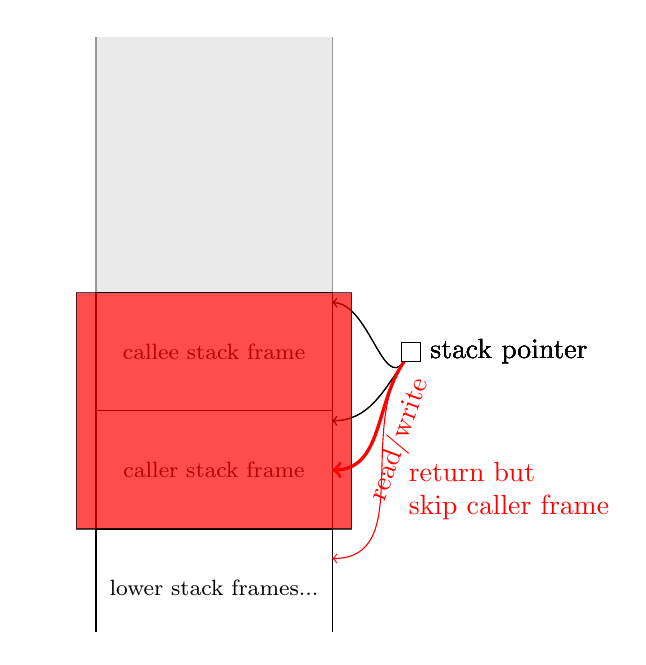
\begin{tikzpicture}[scale=.5, every node={scale=.5}]
    % recurrent parts
    \begin{scope}
      \clip (-.1,-.1) rectangle (6.1,15.1);
      \fill[gray!20,draw=none,opacity=.8] (0,0) rectangle (6,15);
      \draw[draw=gray!80] (0,0) -- (0,15);
      \draw[draw=gray!80] (6,0) -- (6,15);
      \draw[fill=white] (0,-.5) rectangle (6,2.5) node[pos=.5] {\footnotesize lower stack frames...};
    \end{scope}
    \draw (-1.5,0) node {};
    \draw (-1.5,15) node {};
    % \draw[->] (-1,0) -- node[midway,sloped,above] {stack grows upward} (-1,15);

    % traditional:
    \draw<+>[fill=white] (0,2.5) rectangle (6,5.5) node[pos=.5] {\footnotesize caller stack frame};
    \draw<.> (8,7) node[draw=black] (sp0) {};
    \draw<.> node[right=0cm of sp0] (sp0l) { stack pointer };
    \draw<.> (sp0) edge[->,out=235,in=0] (6,5.25);

    % traditional call:
    \draw<+>[fill=white] (0,2.5) rectangle (6,5.5) node[pos=.5] {\footnotesize caller stack frame};
    \draw<.>[fill=white] (0,5.5) rectangle (6,8.5) node[pos=.5] {\footnotesize callee stack frame};
    \draw<.> (8,7) node[draw=black] (sp0) {};
    \draw<.> node[right=0cm of sp0] (sp0l) { stack pointer };
    \draw<.> (sp0) edge[->,out=235,in=0] (6,8.25);

    % traditional return:
    \draw<+>[fill=white] (0,2.5) rectangle (6,5.5) node[pos=.5] {\footnotesize caller stack frame};
    \draw<.> (8,7) node[draw=black] (sp0) {};
    \draw<.> node[right=0cm of sp0] (sp0l) { stack pointer };
    \draw<.> (sp0) edge[->,out=235,in=0] (6,5.25);

    % traditional call, attack:
    \draw<+->[fill=white] (0,2.5) rectangle (6,5.5) node[pos=.5] {\footnotesize caller stack frame};
    \draw<.->[fill=white] (0,5.5) rectangle (6,8.5) node[pos=.5] {\footnotesize callee stack frame};
    \draw<.-> (8,7) node[draw=black] (sp0) {};
    \draw<.-> node[right=0cm of sp0] (sp0l) { stack pointer };

    % read other stack frames
    \draw<.> (sp0) edge[->,out=235,in=0] (6,8.25);
    \actadv[.]{(0,5.5)}{(6,8.5)}{callee stack frame}
    \draw<.> (sp0) edge[->,color=red,very thick,out=235,in=0] node[sloped, below] {read/write} (6,4);

    % break well-bracketedness
    \draw<+>[fill=red,opacity=.7] (-.5,2.5) rectangle (6.5,8.5);
    \draw<.-> (8,7) node[draw=black] (sp0) {};
    \draw<.>[red] (sp0) edge[->,out=235,in=0] (6,1.75);
    \draw<.> node[color=red,align=left,below=of sp0l] {return but\\
      skip caller frame};
  \end{tikzpicture}

\end{frame}

\begin{frame}
  \frametitle{Stack and return capabilities}
  \begin{tikzpicture}[scale=.5, every node={scale=.5}]
    % recurrent parts
    \stdstackstart

    % first step: capabilities
    \begin{onlyenv}<+-+(4)>
      \draw[fill=white] (0,2.5) rectangle (6,5.5) node[pos=.5] {\footnotesize current stack frame};
    \end{onlyenv}
    \begin{onlyenv}<.-.(3)>
      \draw [decorate,decoration={brace,amplitude=10pt,mirror,raise=4pt},yshift=0pt]
      (6.5,2.5) -- (6.5,16) node[draw=black] (sp1) [black,midway,xshift=0.8cm] {};
      \draw node[right=0cm of sp1] { stack pointer };
    \end{onlyenv}
    \begin{onlyenv}<.-.(1)>
      % \draw [decorate,decoration={brace,amplitude=10pt,mirror,raise=4pt},yshift=0pt]
      % (6,0) -- (6,16) node (oldframe1) [black,midway,xshift=0.5cm] {};
      \draw (7.5,4) node[right,fill=gray!50] (rp1l) {return pointer data};
    \end{onlyenv}

    % prepare call: store old return pointer
    \draw<+-+(3)>[fill=gray!50] (0,6) rectangle node {\scriptsize old return pointer code} (6,6.5);
    \begin{onlyenv}<+-+(2)>
      \draw[fill=gray!50] (0,5.5) rectangle node {\scriptsize old return pointer data} (6,6);
      % \draw [decorate,decoration={brace,amplitude=10pt,raise=4pt},yshift=0pt]
      % (0,0) -- (0,16) node (oldframe1) [black,midway,xshift=-0.5cm] {};
      % \draw (0,5.75) edge[->,out=180,in=225] (oldframe1);
    \end{onlyenv}
    \begin{onlyenv}<+->
      \draw [decorate,decoration={brace,amplitude=10pt,mirror,raise=4pt,aspect=.4},yshift=0pt]
      (6,2.5) -- (6,16) node (callerframe1) [draw=black,pos=.4,xshift=0.8cm] {};
      \draw node[fill=gray!50,right=0cm of callerframe1] (rp1l) {new return pointer data};
    \end{onlyenv}
    \begin{onlyenv}<+->
      \draw [decorate,decoration={brace,amplitude=10pt,mirror,raise=4pt},yshift=0pt]
      (6.5,6.5) -- (6.5,16) node[draw=black] (sp1) [black,midway,xshift=0.8cm] {};
      \draw node[right=0cm of sp1] { new stack pointer };
    \end{onlyenv}
    
    % call using capabilities
    \begin{onlyenv}<+->
      \draw[fill=gray!50] (0,2.5) rectangle (6,6.5) node[pos=.5] {\footnotesize caller stack frame};
      \draw[fill=white] (0,6.5) rectangle (6,9.5) node[pos=.5] {\footnotesize callee stack frame};
    \end{onlyenv}
  \end{tikzpicture}
\end{frame}
%%% Local Variables:
%%% TeX-master: "presentation-illustrations"
%%% End:

\begin{frame}<1>[label=sarps]
  \frametitle{Stack and return pointer security}
  \begin{itemize}
  \item Desirable properties:
    \begin{itemize}
    \item Well-bracketed control flow
    \item Stack frame encapsulation
    \end{itemize}
  \item How to enforce?
    \begin{itemize}
    \item Capabilities?
      \begin{itemize}
      \item<2-> Not enough: two attacks!
      \end{itemize}
    \item<3-> CHERI Local capabilities?
      \begin{itemize}
      \item Cannot leave registers
      \item<4-> Works, but... [Skorstengaard et al., ESOP 2018]
      \end{itemize}
    \item<5-> CHERI Linear capabilities?
      \begin{itemize}
      \item Non-copyable capabilities
      \item<6> Works perfectly?
      \end{itemize}
    \end{itemize}
  \end{itemize}
\end{frame}

\section{Stack and return capabilities}
\begin{frame}
  \frametitle{Stack and return capabilities}
  \begin{tikzpicture}[scale=.5, every node={scale=.5}]
    % recurrent parts
    \stdstackstart

    % first step: capabilities
    \begin{onlyenv}<+-+(4)>
      \draw[fill=white] (0,2.5) rectangle (6,5.5) node[pos=.5] {\footnotesize current stack frame};
    \end{onlyenv}
    \begin{onlyenv}<.-.(3)>
      \draw [decorate,decoration={brace,amplitude=10pt,mirror,raise=4pt},yshift=0pt]
      (6.5,2.5) -- (6.5,16) node[draw=black] (sp1) [black,midway,xshift=0.8cm] {};
      \draw node[right=0cm of sp1] { stack capability };
    \end{onlyenv}
    \begin{onlyenv}<.-.(1)>
      % \draw [decorate,decoration={brace,amplitude=10pt,mirror,raise=4pt},yshift=0pt]
      % (6,0) -- (6,16) node (oldframe1) [black,midway,xshift=0.5cm] {};
      \draw (7.5,4) node[right,fill=gray!50] (rp1l) {return capability data};
    \end{onlyenv}

    % prepare call: store old return capability
    \draw<+-+(3)>[fill=gray!50] (0,6) rectangle node {\scriptsize old return cap code} (6,6.5);
    \begin{onlyenv}<+-+(2)>
      \draw[fill=gray!50] (0,5.5) rectangle node {\scriptsize old return cap data} (6,6);
      % \draw [decorate,decoration={brace,amplitude=10pt,raise=4pt},yshift=0pt]
      % (0,0) -- (0,16) node (oldframe1) [black,midway,xshift=-0.5cm] {};
      % \draw (0,5.75) edge[->,out=180,in=225] (oldframe1);
    \end{onlyenv}
    \begin{onlyenv}<+->
      \draw [decorate,decoration={brace,amplitude=10pt,mirror,raise=4pt,aspect=.4},yshift=0pt]
      (6,2.5) -- (6,16) node (callerframe1) [draw=black,pos=.4,xshift=0.8cm] {};
      \draw node[fill=gray!50,right=0cm of callerframe1] (rp1l) {new return capability data};
    \end{onlyenv}
    \begin{onlyenv}<+->
      \draw [decorate,decoration={brace,amplitude=10pt,mirror,raise=4pt},yshift=0pt]
      (6.5,6.5) -- (6.5,16) node[draw=black] (sp1) [black,midway,xshift=0.8cm] {};
      \draw node[right=0cm of sp1] { new stack capability };
    \end{onlyenv}
    
    % call using capabilities
    \begin{onlyenv}<+->
      \draw[fill=gray!50] (0,2.5) rectangle (6,6.5) node[pos=.5] {\footnotesize caller stack frame};
      \draw[fill=white] (0,6.5) rectangle (6,9.5) node[pos=.5] {\footnotesize callee stack frame};
    \end{onlyenv}
  \end{tikzpicture}
\end{frame}

%%% Local Variables:
%%% TeX-master: "presentation-illustrations"
%%% End:

\section{Capabilities are not enough}
\againframe<2>{sarps}
\begin{frame}
  \frametitle{Stack and return capabilities: Attack 1}
  \begin{tikzpicture}[scale=.5, every node={scale=.5}]
    % recurrent parts
    \stdstackstart

    % attacker...
    \begin{onlyenv}<+-+(2)>
      \draw[fill=gray!50] (0,2.5) rectangle (6,6.5) node[pos=.5] {\footnotesize caller stack frame};
      \actadv{(0,6.5)}{(6,9.5)}{callee stack frame}
      \draw [decorate,decoration={brace,amplitude=10pt,mirror,raise=4pt},yshift=0pt]
      (6.5,6.5) -- (6.5,16) node[draw=black] (sp1) [black,midway,xshift=0.8cm] {};
      \draw node[right=0cm of sp1] { stack pointer };
    \end{onlyenv}

    % stores stack pointer in heap
    \begin{onlyenv}<+->
      \begin{scope}
        \fill[gray!20] (14,6) rectangle (18,13);
        \draw (14,6) -- (14,13);
        \draw (18,6) -- (18,13);
      \end{scope}
      \draw (16,14) node {heap memory};
      \draw[fill=gray!50] (14,8) rectangle node[color=red] {\scriptsize copy of old sp} (18,8.5);
    \end{onlyenv}
    \draw<.> (14,8.25) edge[->,red,thick,bend left] (sp1);
    \begin{onlyenv}<+->
      \draw [decorate,decoration={brace,amplitude=10pt,mirror,raise=4pt},yshift=0pt]
      (11.5,6.5) -- (11.5,16) node[draw=black] (spold) [black,midway,xshift=0.8cm] {};
      \draw (14,8.25) edge[->,red,thick,bend left] (spold);
    \end{onlyenv}

    % attacker returns
    \begin{onlyenv}<+>
      \draw [decorate,decoration={brace,amplitude=10pt,mirror,raise=4pt},yshift=0pt]
      (6.5,2.5) -- (6.5,16) node[draw=black] (sp1) [black,midway,xshift=0.8cm] {};
      \draw node[right=0cm of sp1] { stack pointer };
      \draw[fill=white] (0,2.5) rectangle (6,6.5) node[pos=.5] {\footnotesize current stack frame};
    \end{onlyenv}

    % attacker gets called again + uses old stack pointer.
    \begin{onlyenv}<+>
      \draw[fill=gray!50] (0,2.5) rectangle (6,10.5) node[pos=.5] {\footnotesize caller stack frame};
      \actadv{(0,10.5)}{(6,13.5)}{callee stack frame}
      \draw (14,8.25) edge[->,color=red,very thick,out=235,in=0] node[sloped, below] {read/write} (6,8);
      \draw [decorate,decoration={brace,amplitude=10pt,mirror,raise=4pt},yshift=0pt]
        (6.5,10.5) -- (6.5,16) node[draw=black] (sp1) [black,midway,xshift=0.8cm] {};
      \draw node[right=0cm of sp1] { stack pointer };
      % \draw [decorate,decoration={brace,amplitude=10pt,mirror,raise=4pt},yshift=0pt]
      % (6,2.5) -- (6,16) node (callerframe1) [draw=black,midway,xshift=0.8cm] {};
      % \draw node[fill=gray!50,right=0cm of callerframe1] (rp1l) {return pointer data};
    \end{onlyenv}
  \end{tikzpicture}
\end{frame}

\begin{frame}
  \frametitle{Stack and return capabilities: Attack 2}
  \begin{tikzpicture}[scale=.5, every node={scale=.5}]
    % recurrent parts
    \stdstackstart

    % first step: capabilities
    \begin{onlyenv}<+>
      \draw[fill=white] (0,2.5) rectangle (6,4) node[pos=.5] {\footnotesize current stack frame};
      \draw [decorate,decoration={brace,amplitude=10pt,mirror,raise=4pt},yshift=0pt]
        (6.5,2.5) -- (6.5,16) node[draw=black] (sp1) [black,midway,xshift=0.8cm] {};
      \draw node[right=0cm of sp1] { stack pointer };
      % \draw [decorate,decoration={brace,amplitude=10pt,mirror,raise=4pt},yshift=0pt]
      % (6,0) -- (6,16) node (oldframe1) [black,midway,xshift=0.5cm] {};
      % \draw node[fill=gray!50,right=0cm of oldframe1] (rp1l) {return pointer data};
    \end{onlyenv}

    % attacker stores copy of stack pointer high in the stack
    \draw<+->[fill=gray!50] (0,2.5) rectangle (6,4) node[pos=.5] {\footnotesize caller stack frame};
    \begin{onlyenv}<.-.(2)>
      \actadv{(0,4)}{(6,7)}{callee stack frame}
      \draw [decorate,decoration={brace,amplitude=10pt,mirror,raise=4pt},yshift=0pt]
        (6.5,4) -- (6.5,16) node[draw=black] (sp1) [black,midway,xshift=0.8cm] {};
      \draw node[right=0cm of sp1] { stack pointer };
    \end{onlyenv}
    \draw<+->[fill=white] (0,13) rectangle (6,13.5) node[pos=.5,color=red] {\footnotesize copy of sp};
    \draw<.> (6,13.25) edge[red,thick,->,in=45] (sp1);
    \begin{onlyenv}<+->
      \draw [decorate,decoration={brace,amplitude=10pt,mirror,raise=4pt},yshift=0pt]
        (13.5,4) -- (13.5,16) node[draw=black] (spold) [black,midway,xshift=0.8cm] {};
      \draw (6,13.25) edge[red,thick,->,in=45] (spold);
    \end{onlyenv}

    % attacker calls trusted code again
%    \draw<+->[fill=gray!50] (0,4) rectangle (6,7) node[pos=.5] {\footnotesize callee stack frame};
    \begin{onlyenv}<+->
      \inactadv{(0,4)}{(6,7)}{callee stack frame}
    \end{onlyenv}
    \begin{onlyenv}<.>
      \draw[fill=white] (0,7) rectangle (6,9) node[pos=.5] {\footnotesize callee (2) stack frame};
      \draw [decorate,decoration={brace,amplitude=10pt,mirror,raise=4pt},yshift=0pt]
        (6.5,7) -- (6.5,16) node[draw=black] (sp1) [black,midway,xshift=0.8cm] {};
      \draw node[right=0cm of sp1] { stack pointer };
    \end{onlyenv}

    % attacker uses old stack pointer
    \draw<+->[fill=gray!50] (0,7) rectangle (6,9) node[pos=.5] {\footnotesize callee (2) stack frame};
    \begin{onlyenv}<.-.(1)>
      \actadv{(0,9)}{(6,12)}{callee (3) stack frame}
      \draw [decorate,decoration={brace,amplitude=10pt,mirror,raise=4pt},yshift=0pt]
      (6.5,9) -- (6.5,16) node[draw=black] (sp1) [black,midway,xshift=0.8cm] {};
      \draw node[right=0cm of sp1] { stack pointer };
    \end{onlyenv}
    \draw<+> (spold) edge[->,color=red,very thick,out=235,in=0] node[sloped, below] {read/write} (6,8);
  \end{tikzpicture}
\end{frame}

\begin{frame}
  \frametitle{Stack Capabilities Problems}
  \begin{itemize}
  \item Stack capabilities are not a panacea
  \item Stack pointers must not leave stack frame (through memory or stack)
  \item Similar problems for return pointers (omitted)
  \item Solution: local capabilities?
    \begin{itemize}
    \item Make stack and return capabilities local
    \item Cannot leave registers (except on stack) (\sout{Attack 1})
    \item Stack clearing on boundary crossings (\sout{Attack 2})
    \end{itemize}
  \end{itemize}
\end{frame}

\begin{frame}
  \begin{tikzpicture}[scale=.5, every node={scale=.5}]
    \frametitle{Stack and return capabilities: Attack 3}
    \begin{scope}
    \clip (-.1,-.1) rectangle (5.1,10.1);
    \fill[fill=gray!50] (0,0) rectangle (5,10);
    \draw (0,0) -- (0,10);
    \draw (5,0) -- (5,10);
    \end{scope}
    \draw (2.5,11) node {heap memory};

    \begin{scope}
    \clip (12.9,-.1) rectangle (18.1,11.1);
    \fill[fill=gray!50] (13,0) rectangle (18,11);
    \draw (13,0) -- (13,11);
    \draw (18,0) -- (18,11);
    \end{scope}
    \draw (15.5,12) node {more heap memory}; 


    \draw<+->[fill=white] (0,1) rectangle (5,4) node[pos=.5] {\footnotesize caller code};


    \begin{onlyenv}<+->
      \capbrace[ret1]{(5.1,1)}{(5.1,4)}
      \draw node[fill=gray!50, right=0cm of ret1] { \phantom{ret-ptr} };
      \draw node[right=0cm of ret1] { ret-ptr };
    \end{onlyenv}

    \begin{onlyenv}<+->
      \draw[fill=gray!30] (0,1) rectangle (5,4) node[pos=.5] {\footnotesize caller code};
      \draw[fill=white] (13,3) rectangle (18,6) node[pos=.5] {\footnotesize callee code};
      \draw[fill=white] (13,1) rectangle (18,1.5) node[pos=.5] {};
    \end{onlyenv}

    \begin{onlyenv}<.-.(2)>
      \draw [decorate,decoration={brace,amplitude=2pt,mirror,raise=4pt},yshift=0pt]
      (18.1,1) -- (18.1,1.5) node[draw=black] (copy) [black,midway,xshift=0.5cm] {};
      \draw (18,4.75)  edge[->,bend left] (copy);
    \end{onlyenv}

    \begin{onlyenv}<+->
      \draw[fill=white] (13,1) rectangle (18,1.5) node[pos=.5] {\scriptsize {\color{red} copy of ret-ptr}};
      \draw (13,1.25) edge[->,red,thick,bend left] (ret1);
    \end{onlyenv}

    \begin{onlyenv}<+->
      \draw [decorate,decoration={brace,amplitude=10pt,raise=4pt},yshift=0pt]
      (12.9,3) -- (12.9,6) node[draw=black] (ret2) [black,midway,xshift=-0.8cm] {};
      \draw node[fill=gray!50,left=0cm of ret2] { \phantom{ret-ptr (1)} };
      \draw node[left=0cm of ret2] { ret-ptr (1) };
    \end{onlyenv}

    \begin{onlyenv}<+->
      \draw[fill=white] (0,5) rectangle (5,8) node[pos=.5] {\footnotesize callee code (1)};
      \draw[fill=gray!30] (13,3) rectangle (18,6) node[pos=.5] {\footnotesize callee code};
      \draw[fill=gray!30] (13,1) rectangle (18,1.5) node[pos=.5] {\scriptsize {\color{red} copy of ret-ptr}};
    \end{onlyenv}

    \begin{onlyenv}<+->
      \capbrace[ret3]{(5.1,5)}{(5.1,8)}
      \draw node[fill=gray!50,right=0cm of ret3] { \phantom{ret-ptr (2)} };
      \draw node[right=0cm of ret3] { ret-ptr (2) };
    \end{onlyenv}

    \begin{onlyenv}<+->
      \draw[fill=gray!30] (0,5) rectangle (5,8) node[pos=.5] {\footnotesize callee code (1)};
      \draw[fill=white] (13,7) rectangle (18,10) node[pos=.5] {\footnotesize callee code (2)};
    \end{onlyenv}

    \begin{onlyenv}<+->
      \draw (21,7.5) node[devil,opaque=0.5,mirrored,minimum size=1cm] {};
    \end{onlyenv}

    \begin{onlyenv}<+->
      \draw [decorate,decoration={brace,amplitude=2pt,mirror,raise=4pt},yshift=0pt]
      (18.1,1) -- (18.1,1.5) node[draw=black] (copy) [black,midway,xshift=0.5cm] {};
      \draw (18,8.25)  edge[->,red,thick,bend left] (copy);
      \draw[fill=white] (13,1) rectangle (18,1.5) node[pos=.5] {\scriptsize {\color{red} copy of ret-ptr}};
    \end{onlyenv}

    \begin{onlyenv}<+->
      \draw[fill=gray!30] (13,7) rectangle (18,10) node[pos=.5] {\footnotesize callee code (2)};
      \draw[fill=white] (0,1) rectangle (5,4) node[pos=.5] {\footnotesize caller code};
      \draw[fill=gray!30] (13,1) rectangle (18,1.5) node[pos=.5] {\scriptsize {\color{red} copy of ret-ptr}};
    \end{onlyenv}


    \begin{onlyenv}<+->
      \draw (9,5.5) node [ellipse, draw, red, thick,minimum height=1.5cm, minimum width=3cm] { };
      \draw node[red,cloud,cloud puffs=10.8,cloud puff arc=110, aspect=3, draw, fill=white, align=center] () at (12,10) { These were skipped!};  
    \end{onlyenv}
  \end{tikzpicture}
\end{frame}
%%% Local Variables:
%%% TeX-master: "presentation-illustrations"
%%% End:

\section{Local stack and return capabilities}
\againframe<3>{sarps}
\begin{frame}
  \frametitle{Local Stack Capabilities prevent Attack 1}
  \begin{tikzpicture}[scale=.5, every node={scale=.5}]
    % recurrent parts
    \stdstackstart
    
    % attacker...
    \draw[fill=gray!50] (0,2.5) rectangle (6,6.5) node[pos=.5] {\footnotesize caller stack frame};
    \actadv{(0,6.5)}{(6,9.5)}{callee stack frame}
    \draw [decorate,decoration={brace,amplitude=10pt,mirror,raise=4pt},yshift=0pt]
      (6.5,6.5) -- (6.5,16) node[draw=black] (sp1) [black,midway,xshift=0.8cm] {};
    \draw node[right=0cm of sp1] { stack pointer };

    % stores stack pointer in heap
    \begin{scope}
      \fill[gray!20] (14,6) rectangle (18,13);
      \draw (14,6) -- (14,13);
      \draw (18,6) -- (18,13);
    \end{scope}
    \draw (16,14) node {heap memory};
    \draw[fill=gray!50] (14,8) rectangle node[color=red] {\scriptsize copy of old sp} (18,8.5);
    \draw (14,8.25) edge[->,red,thick,bend left] (sp1);
    \draw[teal,very thick] (13.5,7.5) -- (18.5,9);
    \draw[teal,very thick] (18.5,7.5) -- (13.5,9);
    \draw node[teal,cloud,cloud puffs=10.8,cloud puff arc=110, aspect=3, draw, fill=white] () at (14,4) {Stack pointer is local!};  
\end{tikzpicture}
\end{frame}

\begin{frame}
  \frametitle{Local caps: Stack clearing prevents Attack 2}
  \begin{tikzpicture}[scale=.5, every node={scale=.5}]
    % recurrent parts
    \stdstackstart

    % attacker stores copy of stack pointer high in the stack
    \draw[fill=gray!50] (0,2.5) rectangle (6,4) node[pos=.5] {\footnotesize caller stack frame};
    \begin{onlyenv}<+>
      \actadv{(0,4)}{(6,7)}{callee stack frame}
    \end{onlyenv}
    \draw<.-.(2)>[fill=white] (0,13) rectangle (6,13.5) node[pos=.5,color=red] {\footnotesize copy of sp};
    \draw<.-.(2)> [decorate,decoration={brace,amplitude=10pt,mirror,raise=4pt},yshift=0pt]
    (13.5,4) -- (13.5,16) node[draw=black] (spold) [black,midway,xshift=0.8cm] {};
    \draw<.-.(2)> (6,13.25) edge[red,thick,->,in=45] (spold);

    % attacker calls trusted code again
    \begin{onlyenv}<+->
      \inactadv{(0,4)}{(6,7)}{callee stack frame}
    \end{onlyenv}
    \begin{onlyenv}<.-.(1)>
      \draw[fill=white] (0,7) rectangle (6,9) node[pos=.5] {\footnotesize callee (2) stack frame};
      \draw [decorate,decoration={brace,amplitude=10pt,mirror,raise=4pt},yshift=0pt]
        (6.5,7) -- (6.5,16) node[draw=black] (sp1) [black,midway,xshift=0.8cm] {};
      \draw node[right=0cm of sp1] { stack pointer };
    \end{onlyenv}

    % trusted code clears the stack
    \begin{onlyenv}<+->
      \foreach \x in {9,9.5,...,14}
      {
        \draw[fill=white] (0,\x) rectangle (6,\x+.5) node[pos=.5,color=teal] {\footnotesize 0};
      };
    \end{onlyenv}
    \draw<.>[very thick,color=teal] (10,13.5) -- (13,14.5)
    (13,13.5) -- (10,14.5);
    
    % attacker uses old stack pointer
    \draw<+->[fill=gray!50] (0,7) rectangle (6,9) node[pos=.5] {\footnotesize callee (2) stack frame};
    \begin{onlyenv}<.>
      \actadv{(0,9)}{(6,12)}{callee (3) stack frame}
      \draw [decorate,decoration={brace,amplitude=10pt,mirror,raise=4pt},yshift=0pt]
      (6.5,9) -- (6.5,16) node[draw=black] (sp1) [black,midway,xshift=0.8cm] {};
      \draw node[right=0cm of sp1] { stack pointer };
    \end{onlyenv}

    % attacker returns
    \draw<+>[fill=white] (0,9) rectangle (6,12) node[pos=.5] {?};
    \begin{onlyenv}<.>
      \draw[fill=white] (0,7) rectangle (6,9) node[pos=.5] {\footnotesize callee (2) stack frame};
      \draw [decorate,decoration={brace,amplitude=10pt,mirror,raise=4pt},yshift=0pt]
        (6.5,7) -- (6.5,16) node[draw=black] (sp1) [black,midway,xshift=0.8cm] {};
      \draw node[right=0cm of sp1] { stack pointer };
    \end{onlyenv}

    % trusted code clears stack again
    \begin{onlyenv}<+->
      \foreach \x in {7,7.5,...,14}
      {
        \draw[fill=white] (0,\x) rectangle (6,\x+.5) node[pos=.5,color=teal] {\footnotesize 0};
      };
    \end{onlyenv}
    % then, the trusted code can return
    \begin{onlyenv}<+>
      \actadv{(0,4)}{(6,7)}{callee stack frame}
    \end{onlyenv}
    
  \end{tikzpicture}
\end{frame}

\begin{frame}
  \frametitle{Local Stack Capabilities prevent Attack 3}
  \begin{tikzpicture}[scale=.5, every node={scale=.5}]
    % recurrent parts
    \stdstackstart
    
    \begin{scope}
      \fill[gray!50] (13,4) rectangle (18,14);
      \draw (13,4) -- (13,14);
      \draw (18,4) -- (18,14);
      \draw (15.5,15) node {code memory};
    \end{scope}

    \begin{scope}
      \fill[gray!50] (13,0) rectangle (18,2);
      \draw (13,0) -- (13,2);
      \draw (18,0) -- (18,2);
      \draw (15.5,3) node {heap memory};
    \end{scope}

    \begin{onlyenv}<+->
      \actsf{(0,2.5)}{(6,5.5)}{caller stack frame}
      \draw[fill=white] (13,5) rectangle (18,6.5) node[pos=.5] {\footnotesize caller code};
    \end{onlyenv}

\note{Caller calls callee}
\note{Caller clears the stack}
    \begin{onlyenv}<+->
      \foreach \x in {5.5,6,...,14}
      {
        \draw[fill=white] (0,\x) rectangle (6,\x+.5) node[pos=.5,color=teal] {\footnotesize 0};
      };
    \end{onlyenv}

\note{Return pointers always point to the stack as we need to be able to regain the stack pointer itself}
\note{note: the open ended braces are assumed to stretch over the rest of the stack (in the direction it is open)}
    \begin{onlyenv}<+->
      \begin{scope}
        \clip (6.1,2.5) rectangle (8.1,5.5);
        \capbrace[ret1]{(6.1,2.5)}{(6.1,6.5)}
      \end{scope}
      \draw node[fill=gray!50,right=0cm of ret1] { \phantom{ret-ptr} };
      \draw node[right=0cm of ret1] { ret-ptr };
    \end{onlyenv}

    \begin{onlyenv}<+->
      \inactsf{(0,2.5)}{(6,5.5)}{caller stack frame}
      \draw[fill=gray!30] (13,5) rectangle (18,6.5) node[pos=.5] {\footnotesize caller code};
      \draw[fill=white] (13,7) rectangle (18,8.5) node[pos=.5] {\footnotesize callee code};
      \actadv{(0,5.5)}{(6,8.5)}{callee stack frame}
    \end{onlyenv}

\note{Callee cannot store ret-ptr on the heap as it is local!}
    \begin{onlyenv}<+-.(2)>
      \draw (13,1.5) edge[red,bend right,thick,->] (ret1);
    \end{onlyenv}

    \begin{onlyenv}<+>
      \draw[teal,very thick] (11.3,3) -- (13,2.8);
      \draw[teal,very thick] (11.8,3.7) -- (12.4,2);
      \draw node[teal,cloud,cloud puffs=10.8,cloud puff arc=110, aspect=3, draw, fill=white] () at (14,10) {Return pointer is local!};  
    \end{onlyenv}

\note{Callee tries to store ret-ptr on the stack (just like for attack 2)}
    \begin{onlyenv}<+->
      \draw[fill=white] (0,13) rectangle (6,13.5) node[pos=.5,color=red] {\footnotesize copy of sp};
    \end{onlyenv}
    \draw<.> (6,13.25) edge[red,thick,->,in=45] (ret1);

\note{Callee calls callee (1)}
    \begin{onlyenv}<+->
      \begin{scope}
        \clip (6.1,5.5) rectangle (8.1,8.5);
        \capbrace[ret2]{(6.1,5.5)}{(6.1,9.5)}
      \end{scope}
      \draw node[fill=gray!50,right=0cm of ret2] { \phantom{ret-ptr (1)} };
      \draw node[right=0cm of ret2] { ret-ptr (1) };
    \end{onlyenv}
    \draw<.-.(1)> (6,13.25) edge[red,thick,->,in=45] (ret1);

    \begin{onlyenv}<+->
      % \inactsf{(0,2.5)}{(6,5.5)}{caller stack frame}
      \inactadv{(0,5.5)}{(6,8.5)}{callee stack frame}
      \actsf{(0,8.5)}{(6,11.5)}{callee stack frame (1)}
      \draw[fill=gray!30] (13,7) rectangle (18,8.5) node[pos=.5] {\footnotesize callee code};
      \draw[fill=white] (13,9) rectangle (18,10.5) node[pos=.5] {\footnotesize callee code (1)};
    \end{onlyenv}

\note{Callee (1) clears the stack erasing the copy of the ret-ptr!}
    \begin{onlyenv}<+->
      \foreach \x in {11.5,12,...,14}
      {
        \draw[fill=white] (0,\x) rectangle (6,\x+.5) node[pos=.5,color=teal] {\footnotesize 0};
      };
    \end{onlyenv}

\note{Callee (1) calls callee (2)}
    \begin{onlyenv}<+->
      \begin{scope}
        \clip (6.1,8.5) rectangle (8.1,11.5);
        \capbrace[ret3]{(6.1,8.5)}{(6.1,12.5)}
      \end{scope}
      \draw node[fill=gray!50,right=0cm of ret3] { \phantom{ret-ptr (2)} };
      \draw node[right=0cm of ret3] { ret-ptr (2) };
    \end{onlyenv}

    \begin{onlyenv}<+->
      % \inactsf{(0,2.5)}{(6,5.5)}{caller stack frame}
      % \inactadv{(0,5.5)}{(6,8.5)}{callee stack frame}
      \inactsf{(0,8.5)}{(6,11.5)}{callee stack frame (1)}
      \actadv{(0,11.5)}{(6,14.5)}{callee stack frame (2)}
      \draw[fill=gray!30] (13,9) rectangle (18,10.5) node[pos=.5] {\footnotesize callee code (1)};
      \draw[fill=white] (13,11) rectangle (18,12.5) node[pos=.5] {\footnotesize callee code (2)};
    \end{onlyenv}

\note{The copy of ret-ptr callee (2) hoped to use has been erased}
    \begin{onlyenv}<+->
      \draw node[teal,cloud,cloud puffs=10.8,cloud puff arc=110, aspect=3, draw, fill=white, align=center] () at (14,4) {ret-ptr capability gone,\\can only access ret-ptr (2)!};  
    \end{onlyenv}
\end{tikzpicture}
\end{frame}
%%% Local Variables:
%%% TeX-master: "presentation-illustrations"
%%% End:

\againframe<4>{sarps}
\section{Linear stack and return capabilities}
\againframe<5>{sarps}
\begin{frame}
  \frametitle{Linear caps: stack pointers}
  \begin{tikzpicture}[scale=.5, every node={scale=.5}]
    % recurrent parts
    \stdstackstart

    % Caller 
    \actsf{(0,2.5)}{(6,5)}{caller stack frame} 
    \begin{onlyenv}<+>
      \capbrace{(6.5,2.5)}{(6.5,16)}
      \draw node[right=0cm of sp1] { stack pointer };
    \end{onlyenv}


    % Split the stack pointer
    \begin{onlyenv}<+>
      \capbrace[sp2]{(6.5,2.5)}{(6.5,5)}
      \capbrace[usp]{(6.5,5)}{(6.5,16)}
      \draw node[right=0cm of usp] { stack pointer };
      \draw node[right=0cm of sp2] { private stack pointer };
    \end{onlyenv}


    % Callee called
    \begin{onlyenv}<+>
      \capbrace[sp2]{(6.5,2.5)}{(6.5,5)}
      \capbrace[usp]{(6.5,5)}{(6.5,16)}
      \draw node[right=0cm of usp] { stack pointer };
      \draw node[fill=gray!50, right=0cm of sp2] { return data pointer };
      \inactsf{(0,2.5)}{(6,5)}{caller stack frame} 
      \actsf{(0,5)}{(6,6.5)}{callee stack frame}
    \end{onlyenv}

    % Return from callee
    \begin{onlyenv}<+>
      \capbrace[sp2]{(6.5,2.5)}{(6.5,5)}
      \capbrace[usp]{(6.5,5)}{(6.5,16)}
      \draw node[right=0cm of usp] { stack pointer };
      \draw node[right=0cm of sp2] { private stack pointer };
    \end{onlyenv}

    % Caller splices the stack frames
    \begin{onlyenv}<+>
      \capbrace{(6.5,2.5)}{(6.5,16)}
      \draw node[right=0cm of sp1] { stack pointer };
    \end{onlyenv}

  \end{tikzpicture}
\end{frame}

\begin{frame}
    \frametitle{Linear caps prevent attack 1}
  \begin{tikzpicture}[scale=.5, every node={scale=.5}]
    % recurrent parts
    \stdstackstart
    \draw (16.5,5.5) node {register file};
    \begin{scope}
      \clip (15.9,1.1) rectangle (17.1,5.1);
      \foreach \x in {1,2,...,4}
      {
        \draw[fill=white] (16,\x) rectangle (17,\x+1) node[pos=.5,color=teal] {};
      };
    \end{scope}
    \node (r1) at (16.75,4.5) {};
    \node (r2) at (16.75,3.6) {};

    % Caller 
    \actsf{(0,2.5)}{(6,5)}{caller stack frame} 
    \begin{onlyenv}<+>
      \capbrace[sp1]{(6.5,2.5)}{(6.5,16)}
      \draw node[right=0cm of sp1] { stack pointer };
      \draw (r1) edge[->,red,thick,bend left] (sp1);
    \end{onlyenv}


    % Split the stack pointer
    \begin{onlyenv}<+>
      \capbrace[sp2]{(6.5,2.5)}{(6.5,5)}
      \draw (r2) edge[->,red,thick,bend left] (sp2);
      \draw [decorate,decoration={brace,aspect=0.2,amplitude=10pt,mirror,raise=4pt},yshift=0pt]
      (6.5,5) -- (6.5,16) node[draw=black] (usp) [black,pos=0.2,xshift=0.8cm] {};
      \draw (r1) edge[->,red,thick,bend left] (usp);
      \draw node[right=0cm of usp] { stack pointer };
      \draw node[right=0cm of sp2] { private stack pointer };
    \end{onlyenv}


    % Callee called
    \begin{onlyenv}<+>
      \capbrace[sp2]{(6.5,2.5)}{(6.5,5)}
      \draw [decorate,decoration={brace,aspect=0.2,amplitude=10pt,mirror,raise=4pt},yshift=0pt]
      (6.5,5) -- (6.5,16) node[draw=black] (usp) [black,pos=0.2,xshift=0.8cm] {};
      \draw (r1) edge[->,red,bend left] (usp);
      \draw node[right=0cm of usp] { stack pointer };

      \draw node[fill=gray,opacity=0.5, right=0cm of sp2] { \phantom{return data pointer} };
      \draw node[right=0cm of sp2] { return data pointer };
      \inactsf{(0,2.5)}{(6,5)}{caller stack frame} 
      \actadv{(0,5)}{(6,8)}{callee stack frame}
    \end{onlyenv}
    \draw<.-> (r2) edge[->,red,bend left] (sp2);


    \begin{onlyenv}<.->
      \begin{scope}
        \fill[gray!20] (14,9) rectangle (18,14);
        \draw (14,9) -- (14,14);
        \draw (18,9) -- (18,14);
      \end{scope}
    \end{onlyenv}
    \draw<.>[fill=white] (14,10) rectangle node[color=red] {} (18,10.5);

    % Callee stores stack pointer
    \begin{onlyenv}<+->
      \draw [decorate,decoration={brace,aspect=0.2,amplitude=10pt,mirror,raise=4pt},yshift=0pt]
      (8,5) -- (8,16) node[draw=black] (usp) [black,pos=0.2,xshift=0.8cm] {};
      \draw (16,15) node {heap memory};
    \end{onlyenv}

    \begin{onlyenv}<.>
      \draw (14,10.25) edge[->,red,thick,bend right] (usp);
      \draw[fill=white] (14,10) rectangle node[color=red] {\scriptsize old sp} (18,10.5);
      \draw node[right=0cm of usp] { stack pointer };
      \inactsf{(0,2.5)}{(6,5)}{caller stack frame} 
      \actadv{(0,5)}{(6,8)}{callee stack frame}
      \capbrace[sp2]{(6.5,2.5)}{(6.5,5)}
      \draw node[fill=gray,opacity=0.5, right=0cm of sp2] { \phantom{return data pointer} };
      \draw node[right=0cm of sp2] { return data pointer };
    \end{onlyenv}

    % Return from callee
    \begin{onlyenv}<+->
      \draw (14,10.25) edge[->,red,bend right] (usp);
      \draw[fill=gray!50] (14,10) rectangle node[color=red] {\scriptsize old sp} (18,10.5);
      \actsf{(0,2.5)}{(6,5)}{caller stack frame} 
      \capbrace[sp2]{(6.5,2.5)}{(6.5,5)}
      \draw node[right=0cm of sp2] { private stack pointer };
      \draw node[right=0cm of usp] { stack pointer };
    \end{onlyenv}

    \draw<+>[teal,very thick] (6.4,4.4) -- (7.4,5.4);
    \draw<.>[teal,very thick] (7.4,4.4) -- (6.4,5.4);
    \draw<.> node[teal,cloud,cloud puffs=10.8,cloud puff arc=110, aspect=3, draw, fill=white, align=center] () at (14,4) { Splice fails,\\ stack pointer is linear!};  
  \end{tikzpicture}  
\end{frame}

\begin{frame}
  \frametitle{Linear caps prevents attack 2}
  \begin{tikzpicture}[scale=.5, every node={scale=.5}]
    % recurrent parts
    \stdstackstart

    \draw (16.5,5.5) node {register file};
    \begin{scope}
      \clip (15.9,1.1) rectangle (17.1,5.1);
      \foreach \x in {1,2,...,4}
      {
        \draw[fill=white] (16,\x) rectangle (17,\x+1) node[pos=.5,color=teal] {};
      };
    \end{scope}
    \node (r1) at (16.75,4.5) {};
    \node (r2) at (16.75,3.6) {};

    % Caller 
    \actsf{(0,2.5)}{(6,5)}{caller stack frame} 
    \begin{onlyenv}<+>
      \capbrace{(6.5,2.5)}{(6.5,16)}
      \draw node[right=0cm of sp1] { stack pointer };
      \draw (r1) edge[->,red,thick,bend left] (sp1);
    \end{onlyenv}


    % Split the stack pointer
    \begin{onlyenv}<+>
      \capbrace[sp2]{(6.5,2.5)}{(6.5,5)}
      \capbrace[usp]{(6.5,5)}{(6.5,16)}
      \draw (r2) edge[->,red,thick,bend left] (sp2);
      \draw (r1) edge[->,red,thick,bend left] (usp);
      \draw node[right=0cm of usp] { stack pointer };
      \draw node[right=0cm of sp2] { private stack pointer };
    \end{onlyenv}


    % Callee called
    \begin{onlyenv}<+>
      \capbrace[usp]{(6.5,5)}{(6.5,16)}
      \draw (r1) edge[->,red,bend left] (usp);
      \draw node[right=0cm of usp] { stack pointer };
      \inactsf{(0,2.5)}{(6,5)}{caller stack frame} 
      \actadv{(0,5)}{(6,8)}{callee stack frame}
    \end{onlyenv}

    \begin{onlyenv}<.->
      \capbrace[sp2]{(6.5,2.5)}{(6.5,5)}
      \draw node[fill=gray!50,right=0cm of sp2] { \phantom{return data pointer} };
      \draw (r2) edge[->,red,bend left] (sp2);
      \draw node[right=0cm of sp2] { return data pointer };
    \end{onlyenv}

    \begin{onlyenv}<+>

      \capbrace[usp]{(13.5,5)}{(13.5,16)}
      \draw (6,13.25) edge[red,thick,->,in=45] (usp);
      \draw node[right=0cm of usp] { stack pointer };

      \draw[fill=white] (0,13) rectangle (6,13.5) node[pos=.5,color=red] {\footnotesize sp};
      \inactsf{(0,2.5)}{(6,5)}{caller stack frame} 
      \actadv{(0,5)}{(6,8)}{callee stack frame}
    \end{onlyenv}

    % At this point we have a linear point stored in a part of memory that it governs. In other words, no other capabilities can grant access to this part of memory, to the capabilitiy is essentially lost.
%    \draw<+> node[teal,cloud,cloud puffs=10.8,cloud puff arc=110, aspect=3, draw, fill=white, align=center] () at (4,10) { Stack pointer\\essentially lost.}; 

    \begin{onlyenv}<+->

      \capbrace[usp]{(13.5,5)}{(13.5,16)}
      \draw (6,13.25) edge[red,thick,->,in=45] (usp);
      \draw node[right=0cm of usp] { stack pointer };

      \begin{scope}
        \fill[fill=gray!50] (0,2.5) rectangle (6,15) node[pos=.5,color=black] {};
        \draw (0,0) -- (0,15);
        \draw (6,0) -- (6,15);
      \end{scope}
      \draw[fill=gray!50] (0,13) rectangle (6,13.5) node[pos=.5,color=red] {\footnotesize sp};
      \inactsf{(0,2.5)}{(6,5)}{caller stack frame} 
      \inactadv{(0,5)}{(6,8)}{callee stack frame}
      \actsf{(0,8)}{(6,10.5)}{callee (2) stack frame} 
  \end{onlyenv}

  \draw<+>[teal,very thick] (-0.5,7.5) -- (6.5,11);
  \draw<.>[teal,very thick] (-0.5,11) -- (6.5,7.5);
  \draw<.> node[teal,cloud,cloud puffs=10.8,cloud puff arc=110, aspect=3, draw, fill=white, align=center] () at (14,7) { No stack pointer\\for callee (2)!};  

  \end{tikzpicture}
\end{frame}


\begin{frame}
  \frametitle{Linear caps prevents attack 3}
  \begin{tikzpicture}[scale=.5, every node={scale=.5}]
    % recurrent parts
  \scope
    \clip (-.1,-.1) rectangle (6.1,15.1);
    \fill[fill=white] (0,0) rectangle (6,15);
    \draw (0,0) -- (0,15);
    \draw (6,0) -- (6,15);
    \draw[fill=gray!50] (0,-.5) rectangle (6,1.5) node[pos=.5,color=black] {\footnotesize higher stack frames...};
  \endscope
  % \draw[->] (-2,0) -- node[midway,sloped,above] {stack grows upward} (-2,15);
  
  \begin{scope}
    \fill[gray!50] (13,0) rectangle (18,13);
    \draw (13,0) -- (13,13);
    \draw (18,0) -- (18,13);
    \draw (15.5,14) node {code memory};
  \end{scope}

\note{Caller calls callee (split stack pointer to make ret-ptr-d)}
  \begin{onlyenv}<+->
    \actsf{(0,1.5)}{(6,4.5)}{caller stack frame}
    \draw[fill=white] (13,1) rectangle (18,3) node[pos=.5] {\footnotesize caller code};
  \end{onlyenv}
  \begin{onlyenv}<.>
    \capbrace[sp]{(6.1,1.5)}{(6.1,15)}
    \draw node[right=0cm of sp] { sp };
  \end{onlyenv}

  \begin{onlyenv}<+->
    \capbrace[ret1]{(6.1,1.5)}{(6.1,4.5)}
    \draw node[fill=gray!50,right=0cm of ret1] { \phantom{ret-ptr-d} };
    \draw node[right=0cm of ret1] { ret-ptr-d };
  \end{onlyenv}
  \begin{onlyenv}<.->
    \draw [decorate,decoration={brace,aspect=0.3,amplitude=4pt,raise=4pt},yshift=0pt]
    (12.9,1) -- (12.9,3) node[draw=black] (ret1c) [black,pos=0.3,xshift=-0.6cm] {};
    \draw node[fill=gray!50,left=0cm of ret1c] { \phantom{ret-ptr-c} };
    \draw node[left=0cm of ret1c] { ret-ptr-c };
  \end{onlyenv}
 
  \begin{onlyenv}<.-.(3)>
    \capbrace[sp]{(6.1,4.5)}{(6.1,15)}
    \draw node[right=0cm of sp] { sp };
  \end{onlyenv}



  \begin{onlyenv}<+-+(3)>
    \draw[fill=gray!30] (13,1) rectangle (18,3) node[pos=.5] {\footnotesize caller code};
    \draw[fill=white] (13,4) rectangle (18,6) node[pos=.5] {\footnotesize callee code};
    \actadv{(0,4.5)}{(6,7.5)}{callee stack frame}
    \inactsf{(0,1.5)}{(6,4.5)}{caller stack frame}
  \end{onlyenv}

\note{Callee saves ret-ptr-d on the heap.}
  \begin{onlyenv}<+->
    \draw (13,4.75) edge[red,bend right,thick,->] (ret1);
  \end{onlyenv}
\note{Callee saves ret-ptr-c on the heap.}
  \begin{onlyenv}<+->
    \draw (13,4.75) edge[red,bend right,thick,->] (ret1c);
  \end{onlyenv}


\note{Callee calls callee (1)}
\note{Before the callee jumps, it is assumed that it has checked the global "max height" of its stack pointer!}
  \begin{onlyenv}<+-+(4)>
    \capbrace[ret2]{(6.1,4.5)}{(6.1,7.5)}
    \draw node[fill=gray!50,right=0cm of ret2] { \phantom{ret-ptr-d (1)} };
    \draw node[right=0cm of ret2] { ret-ptr-d (1) };
  \end{onlyenv}
  \begin{onlyenv}<.-.(1)>
    \capbrace[sp]{(6.1,7.5)}{(6.1,15)}
    \draw node[right=0cm of sp] { sp };
  \end{onlyenv}

  \begin{onlyenv}<+-+(1)>
    \inactsf{(0,1.5)}{(6,4.5)}{caller stack frame}
    \inactadv{(0,4.5)}{(6,7.5)}{callee stack frame}
    \actsf{(0,7.5)}{(6,10.5)}{callee stack frame (1)}
    \draw[fill=gray!30] (13,1) rectangle (18,3) node[pos=.5] {\footnotesize caller code};
    \draw[fill=gray!30] (13,4) rectangle (18,6) node[pos=.5] {\footnotesize callee code};
    \draw[fill=white] (13,7) rectangle (18,9) node[pos=.5] {\footnotesize callee code (1)};
  \end{onlyenv}

\note{Callee (1) calls callee (2)}
  \begin{onlyenv}<+-+(2)>
    \capbrace[ret3]{(6.1,7.5)}{(6.1,10.5)}
    \draw node[fill=gray!50,right=0cm of ret3] { \phantom{ret-ptr-d (2)} };
    \draw node[right=0cm of ret3] { ret-ptr-d (2) };
  \end{onlyenv}
  \begin{onlyenv}<.->
    \capbrace[sp]{(6.1,10.5)}{(6.1,15)}
    \draw node[right=0cm of sp] { sp };
  \end{onlyenv}

  \begin{onlyenv}<+->
    \inactsf{(0,1.5)}{(6,4.5)}{caller stack frame}
    \inactadv{(0,4.5)}{(6,7.5)}{callee stack frame}
    \inactsf{(0,7.5)}{(6,10.5)}{callee stack frame (1)}
  \end{onlyenv}
  
  \begin{onlyenv}<.->
    \draw[fill=gray!30] (13,1) rectangle (18,3) node[pos=.5] {\footnotesize caller code};
    \draw[fill=gray!30] (13,4) rectangle (18,6) node[pos=.5] {\footnotesize callee code};
    \draw[fill=gray!30] (13,7) rectangle (18,9) node[pos=.5] {\footnotesize callee code (1)};
    \draw[fill=white] (13,10) rectangle (18,12) node[pos=.5] {\footnotesize callee code (2)};
  \end{onlyenv}
  \begin{onlyenv}<.-.(1)>
    \actadv{(0,10.5)}{(6,13.5)}{callee stack frame (2)}
  \end{onlyenv}

\note{Callee (2) has a capability for Callee and can thus access the stored ret-ptr-d}
  \begin{onlyenv}<+->
    \draw [decorate,decoration={brace,amplitude=4pt,mirror,raise=4pt},yshift=0pt]
    (18.1,4) -- (18.1,6) node[draw=black] (calleecap) [black,midway,xshift=0.6cm] {};
    \draw (18,11) edge[red,bend left,thick,->] (calleecap);
  \end{onlyenv}

\note{Callee (2) uses ret-ptr-d to return}
  \begin{onlyenv}<+->
    \actsf{(0,1.5)}{(6,4.5)}{caller stack frame}
    \draw node[fill=white,right=0cm of ret1] { ret-ptr-d };
    \draw node[fill=white,left=0cm of ret1c] { ret-ptr-c };
    \draw (13,4.75) edge[red,bend right,thick,->] (ret1);
  \end{onlyenv}

  \begin{onlyenv}<+->
    \draw<+>[teal,very thick] (6.4,4.4) -- (7.4,5.4);
    \draw<.>[teal,very thick] (7.4,4.4) -- (6.4,5.4);
    \draw<.> node[teal,cloud,cloud puffs=10.8,cloud puff arc=110, aspect=3, draw, fill=white, align=center] () at (10,6) { Splice fails!};  
  \end{onlyenv}
  
\note{Splicing: fails because ends of capabilities don't meet. callee stack frame (1) cannot be empty (it will at least contain 42).}
  % \begin{onlyenv}<+->
  %   \draw node[teal,cloud,cloud puffs=10.8,cloud puff arc=110, aspect=3, draw, fill=white, align=center] () at (8,7.5) {Caller tries to splice sp \\and ret-ptr-d, but fails!};  
  % \end{onlyenv}
\note{Before the caller makes another call/return, it will check that the stack height matches the global max stack height.}
\end{tikzpicture}

\end{frame}

 	
%%% Local Variables:
%%% TeX-master: "presentation-illustrations"
%%% End:
\againframe<6>{sarps}

\begin{frame}
  \frametitle{Formally?}

  \begin{itemize}
  \item<2-> Formulate correctness?
    \begin{itemize}
    % \item<3-> (CFI is too weak (right flows \emph{at the right time}))
    \item<3-> Idea: well-bracketed version of target assembly
    \item<3-> Compiler replaces call/returns with calling convention
    \item<3-> Fully abstract compilation
    \end{itemize}
  \item Prove correctness?
    \begin{itemize}
    \item<4-> Back-translation as embedding
    \item<4-> Cross-language step-indexed Kripke logical relation
    \end{itemize}
  \end{itemize}
\end{frame}

\begin{frame}
  \frametitle{Conclusion}
  \begin{itemize}
  \item Enforcing well-bracketedness and stack frame encapsulation on a capability machine
  \item Local capabilities work [Skorstengaard et al, ESOP 2018]
  \item Linear capabilities work better!
    \begin{itemize}
    \item but don't exist... yet?
    \end{itemize}
  \item Correctness as fully abstract compilation from well-bracketed version of target language.
  \end{itemize}
\end{frame}

\begin{frame}
  \frametitle{Thanks}
  \begin{center}
    \Large Questions?
  \end{center}
\end{frame}

\appendix
\begin{frame}
  \frametitle{Backup slide: The Awkward Example}
  \begin{align*}
    \tau &\isdef (unit \rightarrow unit) \rightarrow int\\
    e_1 &\isdef
          \left\{\begin{aligned}
            &\mathrm{let}~ x~ =~ \mathrm{ref}~ 0~ \mathrm{in}~\\
          &\lambda f\ldotp x \mathrel{:=} 0;~ f~\mathrm{unit}; x \mathrel{:=} 1; f~ \mathrm{unit}; !x
          \end{aligned}\right.\\
    e_2 &\isdef \lambda f\ldotp (f~\mathrm{unit}; f~\mathrm{unit}; 1)
  \end{align*}
\end{frame}

\end{document}
